\label{sec:voltage_rails}

In order to power the components  used in this design, three different voltage
rails are used: \SI{28}{\volt}, \SI{5}{\volt}  and \SI{3.3}{\volt}.  Each rail
has specific  requirements concerning electrical noise,  power and efficiency.
Selecting  appropriate  voltage  regulators requires  determining  approximate
values for the maximum current in each rail.

The power requirements on the \SI{3.3}{\volt} rail are primarily determined by
the dsPIC33  microcontroller and the  LEDs. For maximum processing  power, the
dsPIC33 will  be clocked  at its  maximum frequency  of \SI{120}{\mega\hertz},
consuming  \SI{0.5}{\milli\ampere\per\mega\hertz}  \cite{ref:datasheet:dspic}.
Each of the four LEDs consumes \SI{15}{\milli\ampere}.  This yields a combined
current consumption on the \SI{3.3}{\volt} rail of
\begin{equation}
    I_{\SI{3.3}{\volt}} = I_{dsPIC} + 4 \cdot I_{LED} = \SI{0.5}{\milli\ampere\per\mega\hertz} \cdot \SI{120}{\mega\hertz} + 4 \cdot \SI{15}{\milli\ampere} = \SI{120}{\milli\ampere}\text{.}
\end{equation}

The \SI{5}{\volt}  rail supplies  both the \SI{3.3}{\volt}  rail and  the OLED
display with power. According to  its datasheet \cite{ref:datasheet:oled}, the
OLED display  draws a  maximum current of  \SI{135}{\milli\ampere}. Adding the
current for the \SI{3.3}{\volt} rail yields an approximate current consumption
on the \SI{5}{\volt} line of:

\begin{equation}
    I_{\SI{5}{\volt}} = I_{\SI{3.3}{\volt}} + \SI{135}{\milli\ampere} = \SI{255}{\milli\ampere}
\end{equation}

%Having determined  the current requirements for  each rail, we can  now choose
%appropriate methods  to generate  the voltage and  current. The \SI{28}{\volt}
%rail is provided by the power supply directly.

For  generating  the  lower  voltages from  the  \SI{28}{\volt}  rail,  either
linear regulators  or switch-mode regulators can  be used. Because switch-mode
regulators  are far  more  efficient than  linear  regulators, and  efficiency
depends on the  voltage drop, a switch-mode regulator is  used to convert from
\SI{28}{\volt} to \SI{5}{\volt}.

All  digital  circuitry  operates  on  the  \SI{3.3}{\volt}  rail. Critically,
this  includes  the  microcontroller   and  its  digital-to-analog  (DAC)  and
analog-to-digital   (ADC)  converters. It   is  therefore   crucial  for   the
\SI{3.3}{\volt} rail to have as little  jitter and noise as possible, making a
linear regulator  the preferred  choice for  converting from  \SI{5}{\volt} to
\SI{3.3}{\volt}. A low-quality \SI{3.3}{\volt} rail could lead to inaccuracies
in measuring and regulating output.  The circuits for the two conversions from
\SI{28}{\volt} to \SI{5}{\volt} and  from \SI{5}{\volt} to \SI{3.3}{\volt} are
illustrated in Figure \ref{fig:circuit:rails}.

%The selected  regulator fulfills the
%current requirement and can supply a maximum current of \SI{1}{\ampere}.

\begin{figure}[th!]
    \center
    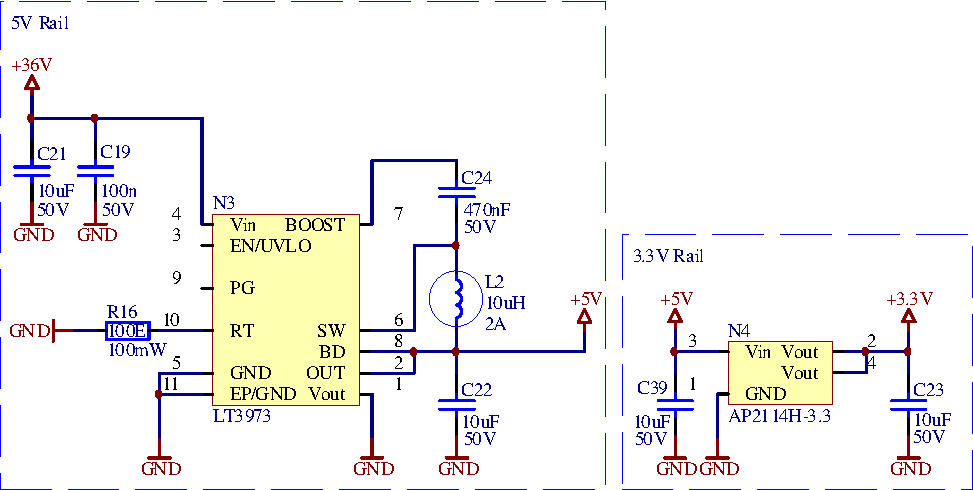
\includegraphics[width=.67\textwidth]{images/circuit/5v-3v-rails.pdf}
    %\caption{Speisung f\"ur 5V mittels Abwertswandler (links) und Speisung f\"ur 3.3V mittels Linearregler (rechts)}
    \caption{Supplying the \SI{5}{\volt} rail via switch-mode regulator (left) and the \SI{3.3}{\volt} rail via linear regulator (right)}
    \label{fig:circuit:rails}
\end{figure}
